\documentclass[12pt]{article}
\usepackage{amsmath}
\usepackage{listings}
\usepackage{graphicx}
\usepackage{caption}
\usepackage{subcaption}
\usepackage{commath}
\usepackage{hyperref}
\usepackage{xcolor}
\usepackage{textcomp}
\usepackage{dirtytalk}
\usepackage{listings,lstautogobble}
\usepackage{xcolor}
\usepackage{wasysym}
\usepackage{float}
\usepackage{mathrsfs}
\usepackage{algpseudocode}
\usepackage{algorithm}
\usepackage{hyperref}


\lstset{language=c++, 
		autogobble=true,
		breaklines = true, 
		   basicstyle=\ttfamily,
           keywordstyle=\color{blue}\ttfamily,
           stringstyle=\color{red}\ttfamily,
           commentstyle=\color{green}\ttfamily}
\begin{document}
\title{Project 4}
\author{Robert Solli}
\maketitle

\section{Introduction}
Through the history of computing a focus has always been on the ability to solve larger and larger systems. Macroscopic thermodynamic systems are no exception. In this project an exploration of the ising model for magnetic spins is explored with a set of small matrices. Initially the focus will be on establishing coherency between analytical and numerical models regarding a small scale system. After which the model is scaled up to consider matrices of a larger size to study steady state systems as well as probability destributions for energies. A final consideration is made for systems with exceedingly large matrices ($140 \times 140$) where parallellization of the code is paramount to the ability to solve the time and temperature evolution of the thermodynamic system.


The code used for the un-parallellized results (all values and plots with $L\leq 20$) can be found at \href{https://github.com/copperwire/project4}{the authors github page}, while the paralellized code can be found at on a \href{https://github.com/geirtul/fys4150_project4}{collaborators github page}.This project has been completed in collaboration with Geir Ulvik and Oda Johanne Kristensen.

\section{Theory}
This project will discuss and implement a solution for the two-dimensional Ising model of ferromagnetism. The model represents a lattice with discrete variables. The lattice can be described using a matrix with the elements being the magnetic dipole moments of atomic spins. The model allows for each spin-site to interact with its neighbour, and is also fertile ground from which to describe phase transitions.

\subsection{A brief cosideration of statistical physics}
The framework for understanding microscopic or quantum systems in large configurations is known colloquially as thermodynamics, or statistical physics. One of the principal sizes in statistical physics  is the partition function $Z$. The shape of the partition function varies depending on the ensemble one operates in. A thermodynamic ensemble defines which pysical sizes are that are constrained within the system. In this project the focus will be on the so called "canonical ensemble" which can exchange energy with the surroundings of the system. In the canonical ensemble the partition function is given as:

\begin{equation}
Z = \sum ^M _{i = 0}  e^{-\beta E_i}
\end{equation}

\noindent Where $\beta = \frac{1}{kT}$ is the inverse temperature of the system by the boltzmann constant. $E_i$ denotes the energy for each unique configuration of the system. It's worthwhile to note that most systems are degenerate in the more common energies. The probability of a given state, which will also serve as a direct analogy to the hamiltonian, is:

\begin{equation}
P(E) = \frac{e^{-\beta E}}{Z}
\end{equation}

\noindent Such that any observable, $A$, has the expectation value 

\begin{equation}
\langle A \rangle = \frac{1}{Z}\sum ^M _{i = 0} A_i e^{- \beta E_i}
\end{equation}

\noindent In addition to expectation values, the variance in observables are often of special interest. In this project the interest will mainly focus on the variance in energy and magnetization given respectively as: 

\begin{equation}
C_v = \frac{1}{kT^2}(\langle E^2 \rangle - \langle E \rangle ^2)
\end{equation}

\begin{equation}\label{eq:chi}
\chi = \beta(\langle \mathscr{M} ^ 2 \rangle - \langle \mathscr{M} \rangle ^2)
\end{equation}


\noindent The potential of the canonical system is the measure of helmholtz free energy, which is defined as:

\begin{equation}
F  = - \frac{1}{\beta} ln Z
\end{equation}

\subsection{An analytical consideration of the two-dimensional ising model}
The two-dimensional Ising model has an energy given by the equation 

\begin{equation}\label{eq:is_ener}
E_i = -J \sum _{<kl>}^N s_k s_l + \mathscr{B} \sum ^N _k s_k 
\end{equation}

\noindent Where $J$ is a coupling constant which determines the strength of the bond between neighbouring spin. The sum over $<kl>$ denotes the neighbouring spins of the site the sum is pointing to in that iteration. In the two dimensional lattice each site has four neighbouring spins, excepting the edge conditions where the number may be three or two for the "corner" elements. The second contribution to the energy is controlled by the magnitued of an externally applied magnetic field, $\mathscr{B}$. 

\noindent The magnetization of the state is given as: 

\begin{equation}
\mathscr{M}_i = \sum^N _{k = 0} s_k
\end{equation}

\subsubsection{The four-spin system}
To ensure that the implementation developed in section \ref{sec:prog_theor} is reasonable an analytical consideration of the $2 \times 2 $ case of the two dimensional ising model is made. For this case the partition function is given as:

\begin{align*}
Z = \sum _{s_i \pm 1} \prod _i e^{\beta j s_i s_{i +1}}
\end{align*}

\noindent that can be explicitly evaluated to 

\begin{align*}
Z &= 4(\frac{e^{8j \beta } + e^{-8j\beta }}{2}) + 12 \\
 & = 4 \cosh{8j \beta} + 12
\end{align*}


\noindent In this case there is no externally applied magnetic field so the second term of the equation \ref{eq:is_ener} dies. As it turns out, the expectation value of the energy can be found by the partial differentiation:

\begin{equation}
\langle E \rangle = \frac{\partial ln Z}{\partial \beta}
\end{equation}

\noindent which is evaluated to 

\begin{align*} 
\langle E \rangle &= \frac{\partial (4 \cosh{8j\beta} +12)}{\partial \beta} \hspace*{0.1in}\frac{\partial ln x}{\partial x} \\
\langle E \rangle  &=  \frac{32 j \sinh{8j \beta} }{Z}
\end{align*}

\noindent further, the variance is in turn the partial derivative 

\begin{equation}
C_v = \frac{1}{kT^2}\frac{\partial ^2 ln Z}{\partial \beta ^2}
\end{equation}

\noindent which can easily be evaluated analytically: 

\begin{align*}
C_v &= \frac{1}{kT^2}\frac{\partial}{\partial \beta}  \frac{32 j \sinh{8j \beta} }{Z}\\
 &= \frac{32j}{kT^2}\frac{\partial }{\partial \beta} \frac{\sinh{8j \beta} }{Z} \\
 &= \frac{32j}{kT^2} \frac{8j\cosh{8j\beta} Z - \partial Z \sinh{8j\beta}}{Z^2} \\
 &= \frac{32j}{kT^2} \left( \frac{8j \cosh{8j \beta}}{Z} - \frac{32 j^2 \sinh ^2 {8j\beta}}{Z^2}\right) \\
 &= \frac{256 \cosh{8j\beta}}{Z} - \langle E \rangle ^2
\end{align*}

\begin{equation}\label{eq:cv}
C_v = \frac{256 \cosh{8j\beta}}{Z} - \langle E \rangle ^2
\end{equation}

\noindent The magnetization of the system is aquired from equation \ref{eq:chi} and can be evaluated directly with relatively low effort since most configurations in the L=2 case have $\mathscr{M}_i = 0$. A small concsession is made for the size of the lattice; 	 the value for $\langle \mathscr{M} \rangle$ fluctuates considerably for small matrices, we'll use the absolute value  $\langle | \mathscr{M} | \rangle$ . 

\begin{align*}
\chi &= \beta(\langle \mathscr{M} ^ 2 \rangle - \langle |\mathscr{M}| \rangle ^2) \\
     &= \frac{1}{Z} \left( \sum ^M _{i = 0} \mathscr{M}_i^2 e^{- \beta E_i} - \frac{1}{Z}\left( \sum ^M _{i = 0} |\mathscr{M}_i| e^{- \beta E_i}\right)^2 \right) \\     
 &= \frac{1}{Z} \left(32e^{8j\beta} + 32 - \frac{1}{Z}\left(8e^{8j\beta + 16}\right)^2 \right)
\end{align*}


\begin{equation}\label{eq:chi}
\chi = \frac{1}{Z} \left(32e^{8j\beta} + 32 - \frac{1}{Z}\left(8e^{8j\beta + 16}\right)^2 \right)
\end{equation}
\subsection{Time evolution of a thermodynamical system}\label{sec:prog_theor}

This project is based on using monte carlo cycles as a representation for time development of a system. A monte-carlo cycle is characterized by a random, or more often, psuedo-random process that govern the logic in the algorithm. The metropolis algoritm which is used to solve this time evolution is based on the probability of  a change in energy of the system. For the two dimensional ising model, this change of energy by flipping one random spin, has a limited set  of outcomes that can be precalculated for increased efficiency. The algorithm is relatively simple and can be stated as \\
\begin{algorithmic}
\Require Establish an initial state of the system with spins arranged with arbitrary direction.
\For{$i \leq \text{ max monte carlo cycles}$ }
	\State Flip one spin 
	\State Compute the energy difference between the original state and the new
	\Comment The energy difference exponential is pre-calculated and used for a lookup
	\If{$r<e^{\Delta E }$}
	\State accept the new configuration
	\EndIf
\EndFor
\end{algorithmic}

The metropolist "if" test ensures that the system will converge to the steady-state oscillating around the expectation values for the system.
\section*{Method}

Implementation of section \ref{sec:prog_theor} as a function written in c++

\begin{lstlisting}

for(int y =0; y < n_spins; y++) {
    for (int x= 0; x < n_spins; x++){

      double r1 = ((double) rand() / (RAND_MAX)) ;
      double r2 = ((double) rand() / (RAND_MAX)) ;
      double r3 = ((double) rand() / (RAND_MAX)) ;

      int ix = (int) (r1 * (double) (n_spins -1));
      int iy = (int) (r2 * (double) (n_spins -1));

      int deltaE = 2*spin_matrix(iy, ix)*
                   (spin_matrix(iy, periodic(ix,n_spins,-1))+
                   spin_matrix(periodic(iy,n_spins,-1), ix) +
                   spin_matrix(iy, periodic(ix,n_spins,1)) +
                   spin_matrix(periodic(iy,n_spins,1), ix));
      if ( r3 <= w[deltaE+8] )
         {
          spin_matrix(iy, ix) *= -1; // flip one spin and accept new spin config
          // update energy and magnetization
          counter_accept += 1;
          M += (double) 2*spin_matrix(iy, ix);
          E += (double) deltaE;
         }

     }
}
\end{lstlisting}

Wherein the array $w$ contains the exponentials corresponding to each energy-delta. The parallelized version of this code leverages splitting the iteration over a temperature-range to different cores on the computer. This segmentation of the program allows for a much speedier computational process for larger lattices.
\section*{Results}

Testing the convergence of the monte-carlo method with the metropolis test is done by implementing a $L = 2$ matrix and iterating for a fairly large number of cycles. The results are then compared with the analytical results by evaluating the equations \ref{eq:cv} and \ref{eq:chi}.

\begin{equation}\label{eq:heat_cap}
C_v = 0.03208
\end{equation}

\begin{equation}\label{eq:mean_magn}
\chi = 0.00401
\end{equation}

After implementing the metropolis algorithm discussed in section \ref{sec:prog_theor} a check was made to ensure coherency in the implementation with the theoretical results from equations \ref{eq:heat_cap} and \ref{eq:mean_magn}. Running the program for $T = 1$ in units of $\frac{kT}{J}$ produces the following output after $10^6$ monte-carlo cycles.

\begin{lstlisting}
Variance in energy: 0.0321814
Variance in magnetization: 0.00399872

Variance in energy: 0.0320874
Variance in magnetization: 0.00401172

Variance in energy: 0.0323233
Variance in magnetization: 0.00402555
\end{lstlisting} 

\noindent As the values are reasonably stable after repeat experiments and are very close to the analytically found values it can be concluded that the method converges for $L = 2$. However, the results are not convincingly stable for a number of cycles of any order of magnitude lower than $10^5$. Building on this framework a consideration of the development of expectation values is made. The continiously developing expectation values for  $C_v$ and $\chi$  and the variance in expectation value for the energy and magnetization.

\begin{figure}
\hspace*{-2cm}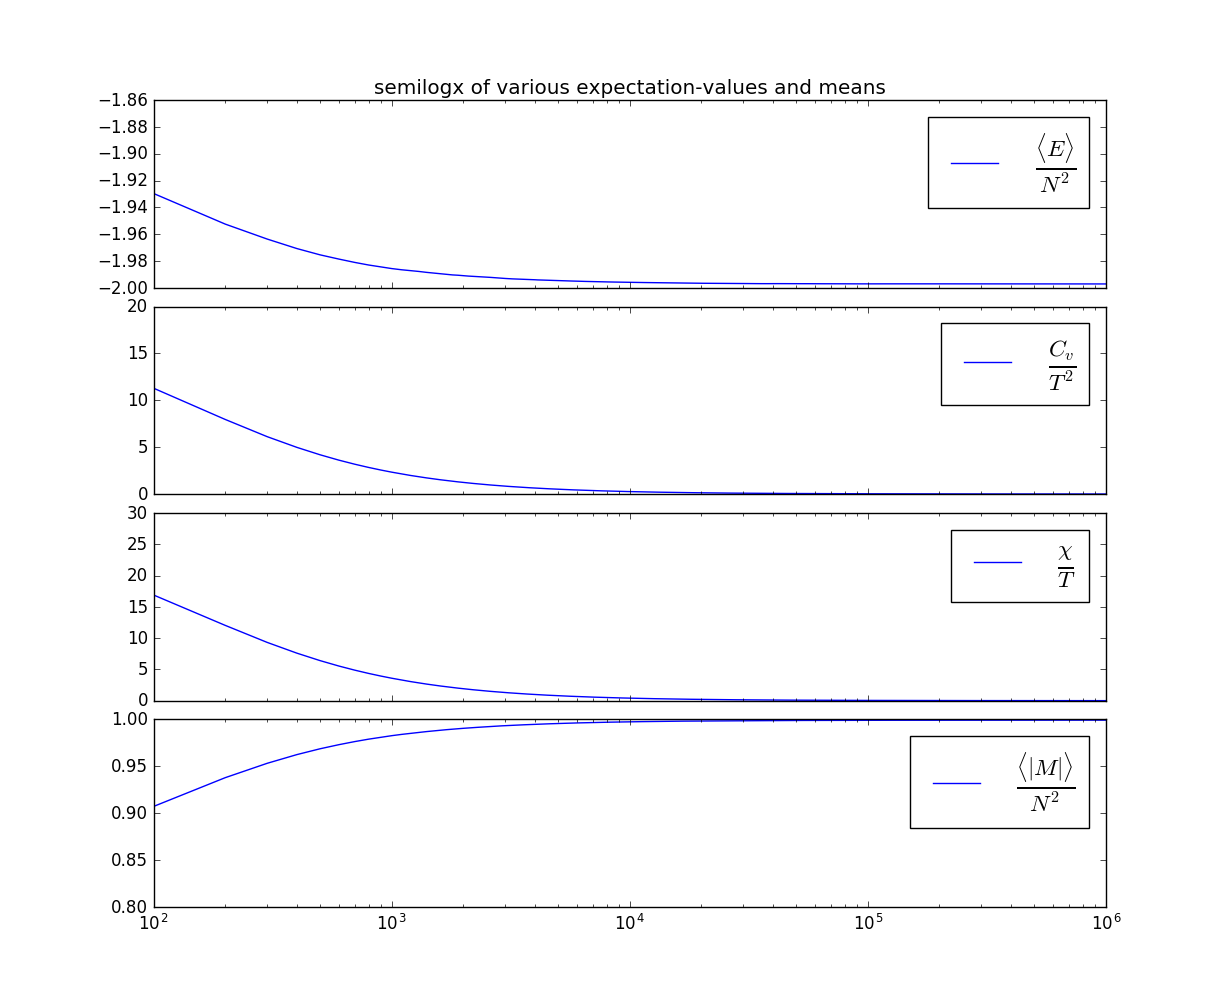
\includegraphics[scale=0.5]{exp_vals.png}
\caption{A set of plots for a temperature $T = 1.0$ and an initial configuration with spins in arbitrary up and down configurations with a lattice size $L = 20$. The x-axis denotes the number of monte carlo cycles and represents the time evolution of the system}\label{fig:exp_t1}
\end{figure}

\begin{figure}
\hspace*{-4cm}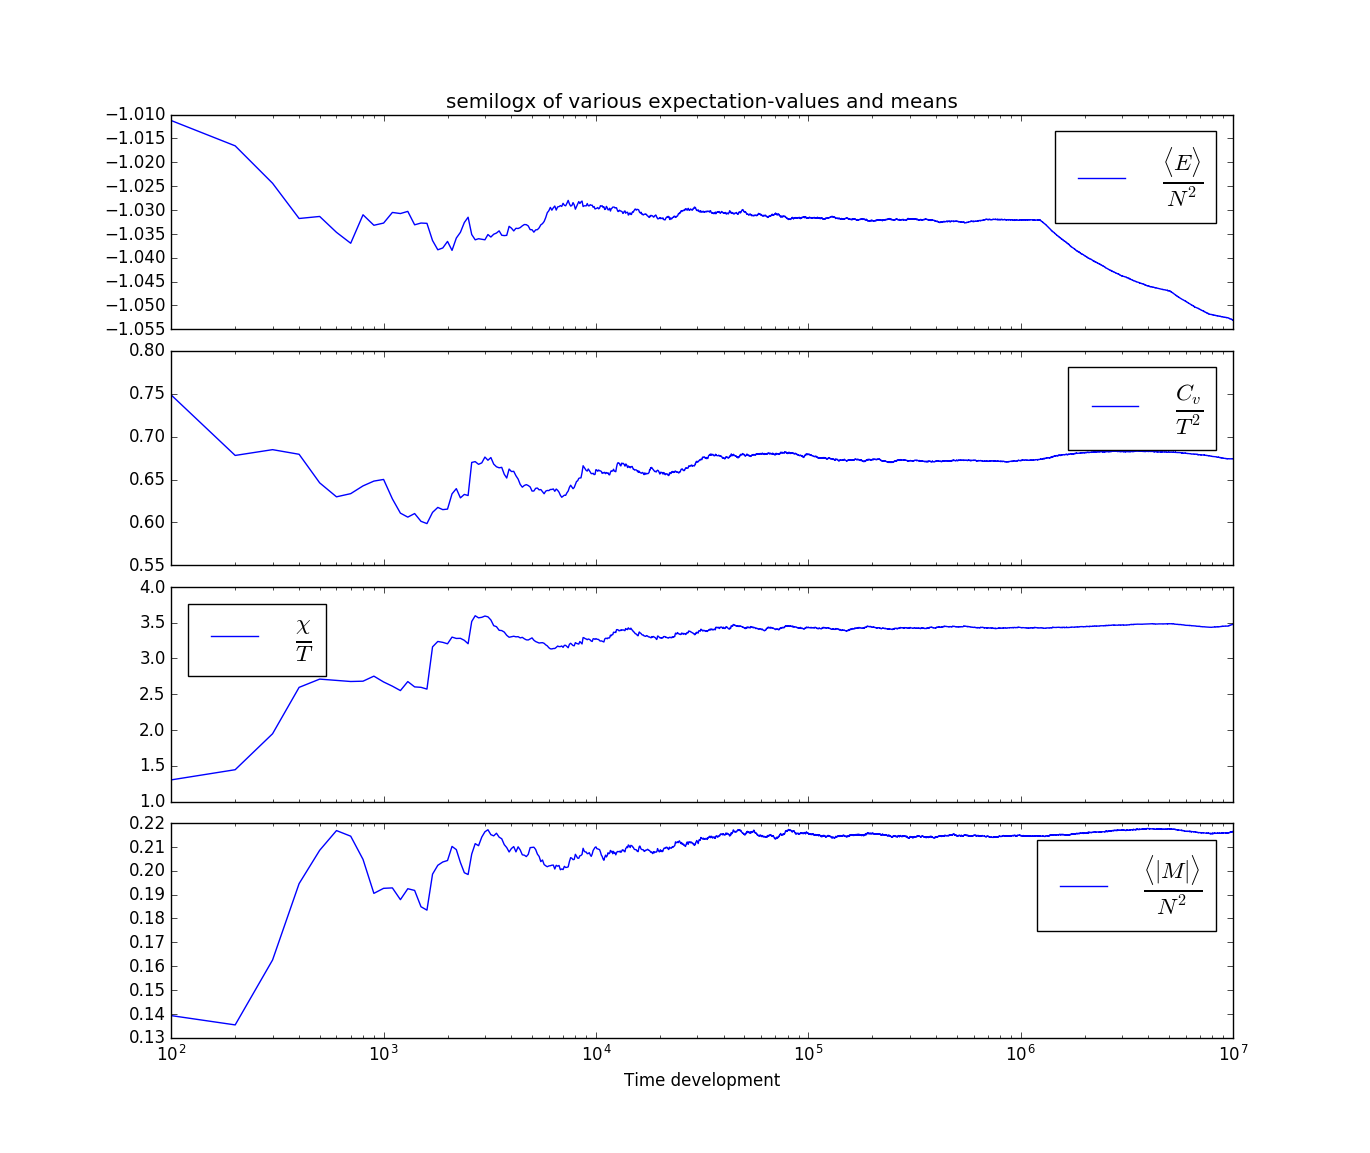
\includegraphics[scale=0.5]{exp_vals_2.png}
\caption{A set of plots for a temperature $T = 2.4$ and an initial configuration with spins in arbitrary up and down configurations with a lattice size $L = 20$. The x-axis denotes the number of monte carlo cycles and represents the time evolution of the system}\label{fig:exp_t2}
\end{figure}


\begin{figure}[H]
\hspace*{-1cm}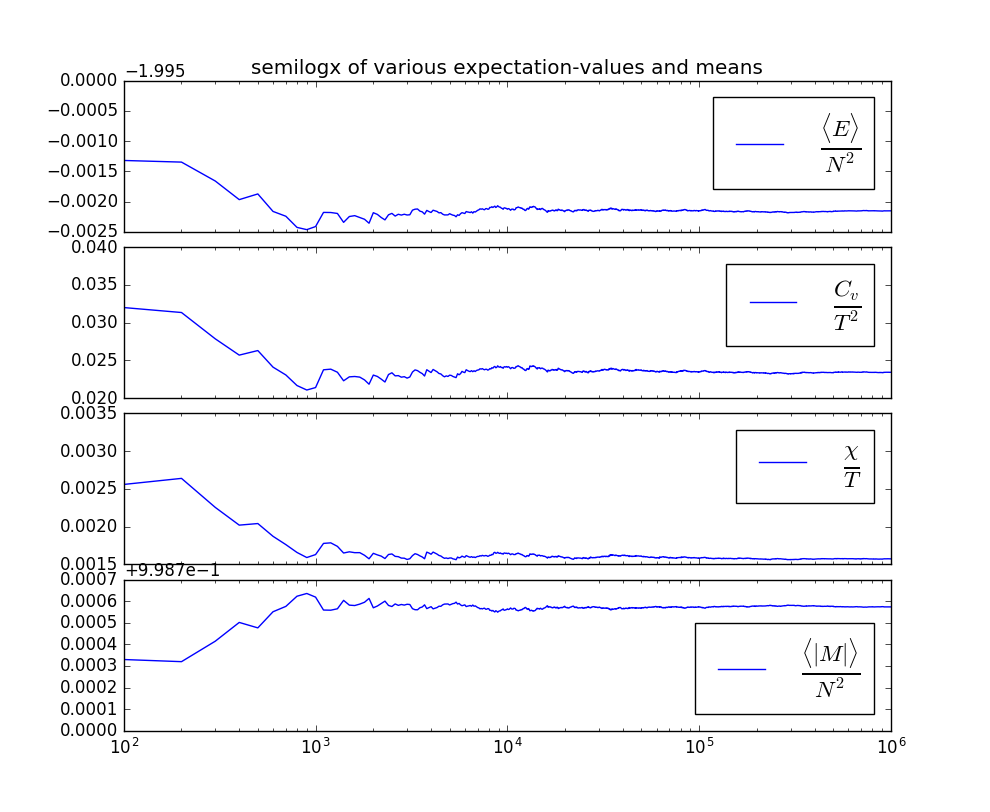
\includegraphics[scale=0.6]{exp_vals_ord_1.png}
\caption{A set of plots for a temperature $T = 1.0$ and an initial configuration with spins all pointing the same direction and a lattice size of $L = 20 $. The x-axis denotes the number of monte carlo cycles and represents the time evolution of the system}\label{fig:exp_t1_ord}
\end{figure}

\begin{figure}[H]
\hspace*{-1cm}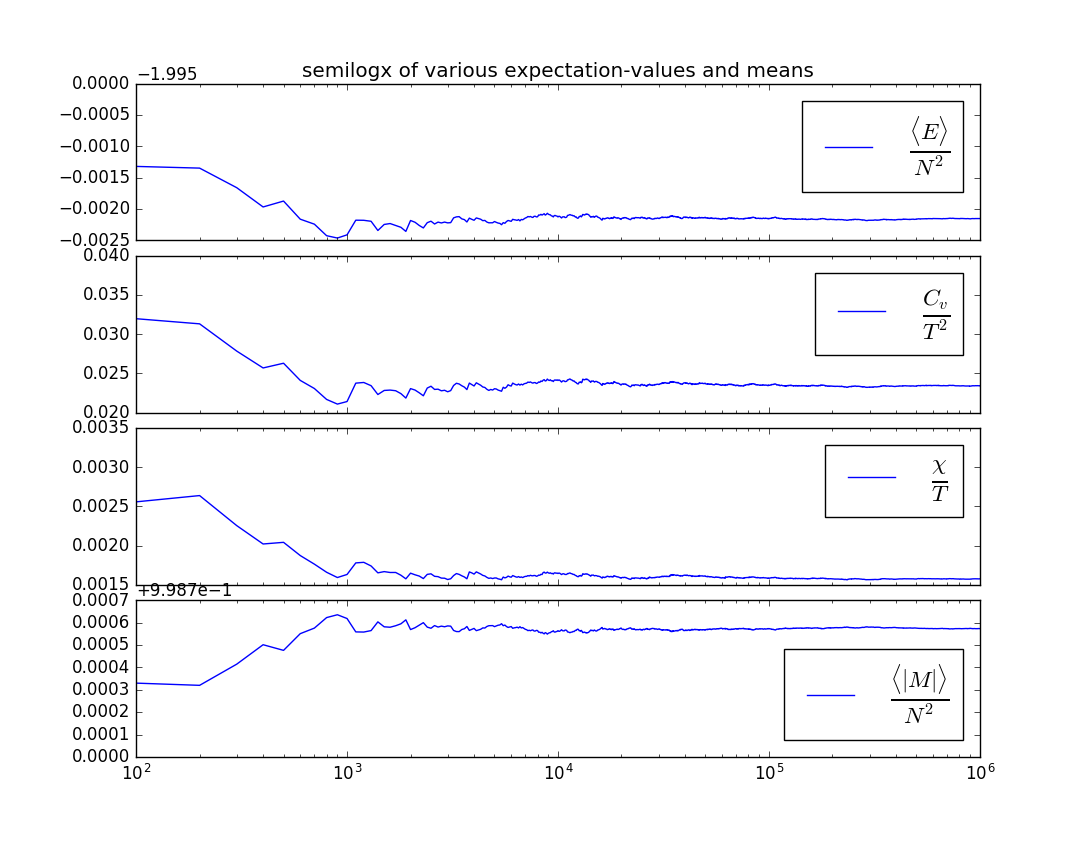
\includegraphics[scale=0.55]{exp_vals_ord_2.png}
\caption{A set of plots for a temperature $T = 2.4$ and an initial configuration with spins all pointing the same direction and a lattice size of $L = 20 $. The x-axis denotes the number of monte carlo cycles and represents the time evolution of the system}\label{fig:exp_t2_ord}
\end{figure}

\iffalse
\begin{figure}[H]
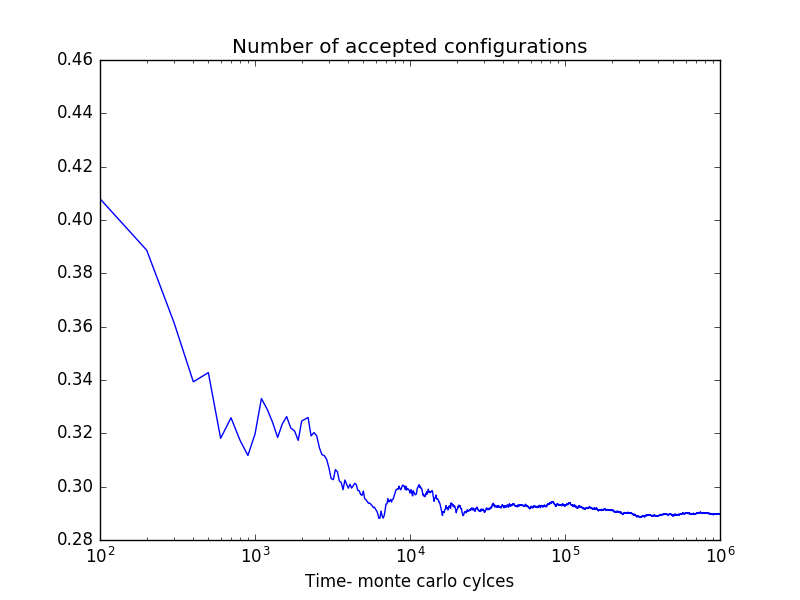
\includegraphics[scale=0.6]{accept_config_ord_1.png}
\caption{Presenting the number of accepted configurations according to the Metropolis test per number of monte - carlo cycles noted on the x-axis. This plot holds for a system with temperature $T = 1.0$, an initial configuration with spins all pointing the same direction and a lattice size of $L = 20 $}\label{fig:accept_config_1_ord}
\end{figure}

\begin{figure}[H]
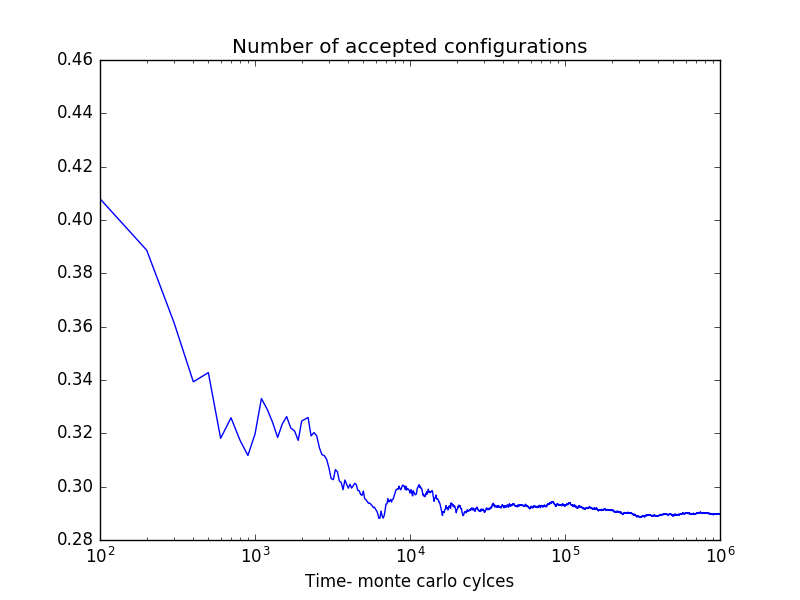
\includegraphics[scale=0.6]{accept_config_ord_2.png}
\caption{Presenting the number of accepted configurations according to the Metropolis test per number of monte - carlo cycles noted on the x-axis. This plot holds for a system with temperature $T = 2.4$, an initial configuration with spins all pointing the same direction, and a lattice size of $L = 20 $}\label{fig:accept_config_ord}
\end{figure}

\begin{figure}[H]
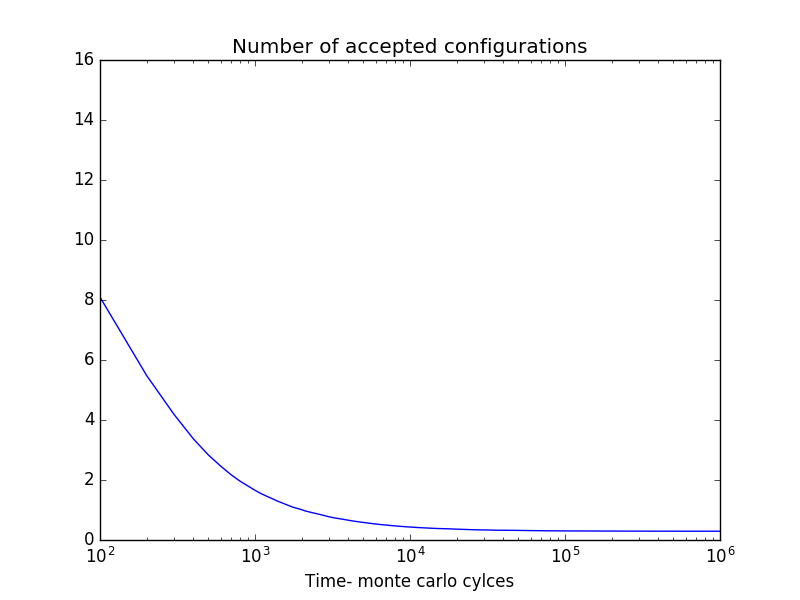
\includegraphics[scale=0.6]{accept_config_1.png}\label{fig:accept_config_1}
\caption{Presenting the number of accepted configurations according to the Metropolis test per number of monte - carlo cycles noted on the x-axis. This plot holds for a system with temperature $T = 1.0$, a configuration with spins in arbitrary states, and a lattice size of $L = 20 $}
\end{figure}

\begin{figure}[H]
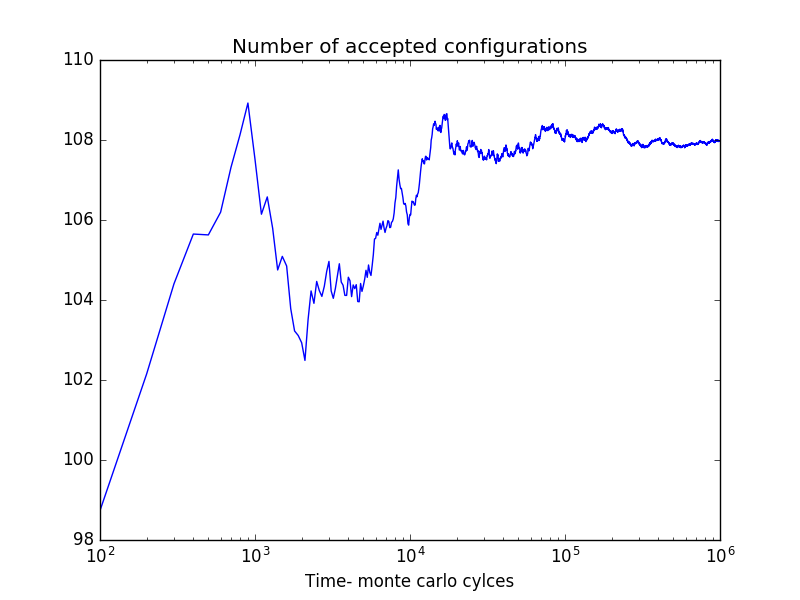
\includegraphics[scale=0.6]{accept_config.png}\label{fig:accept_config}
\caption{Presenting the number of accepted configurations according to the Metropolis test per number of monte - carlo cycles noted on the x-axis. This plot holds for a system with temperature $T = 2.4$, a configuration with spins in arbitrary states, and a lattice size of $L = 20 $}
\end{figure}
\fi


\begin{figure}[H]
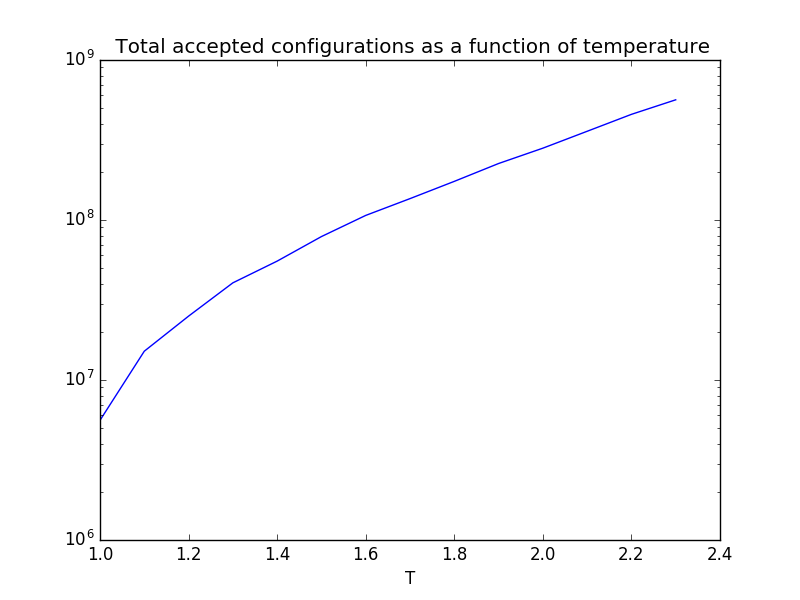
\includegraphics[scale=0.6]{temp_total_config.png}
\caption{A figure of the temperature development of the total number of accepted states in a lattice with $L = 20$}\label{fig:temp_config}
\end{figure}


\begin{figure}[H]
\hspace*{-2cm}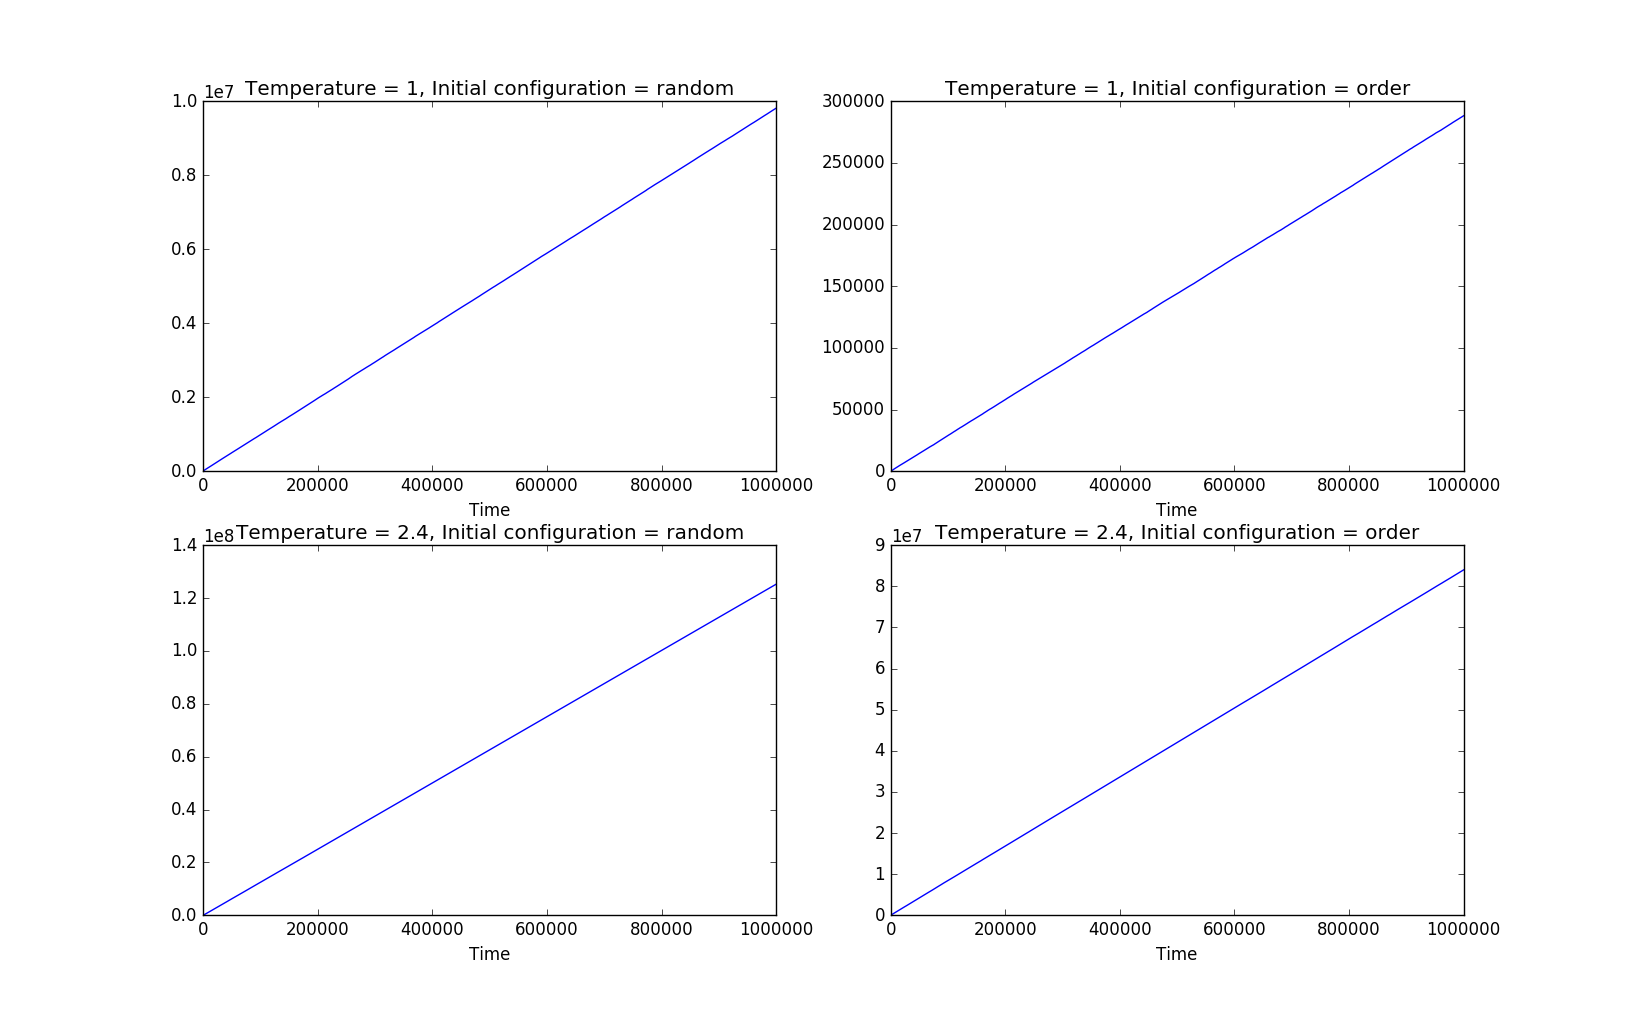
\includegraphics[scale=0.4]{accept_configs.png}
\caption{A set of plots showing the time evolution of the number of accepted states. The plots show the difference in accepted states as a function of temperature and initial state}\label{fig:accept_config}
\end{figure}


\begin{figure}[H]
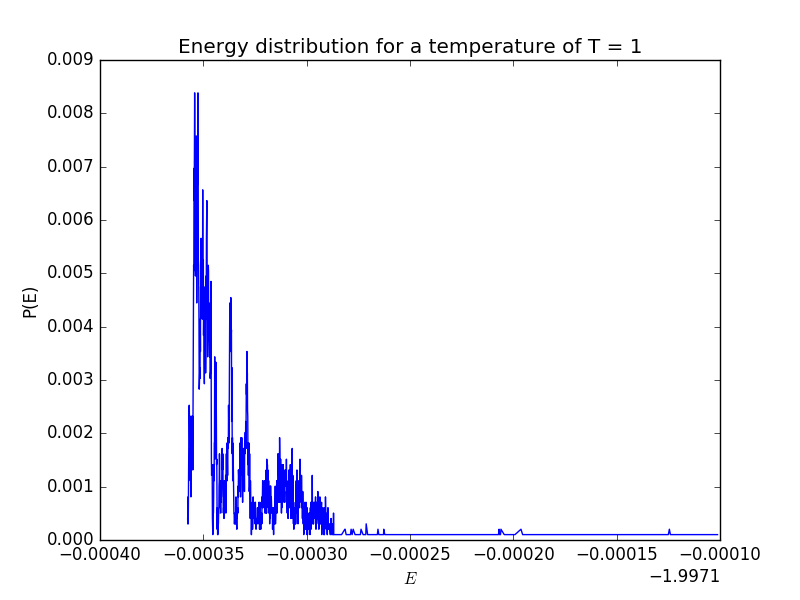
\includegraphics[scale=0.6]{PDF_T_1.png}
\caption{Configuration of the probability density function for energy for a lattice of $L = 20$. The axis is unfortunately partially unreadable because of how close the values are. As it stands the x-ticks should be interpereted as the difference from the lower right number}\label{fig:pdf_1}
\end{figure}

\begin{figure}[H]
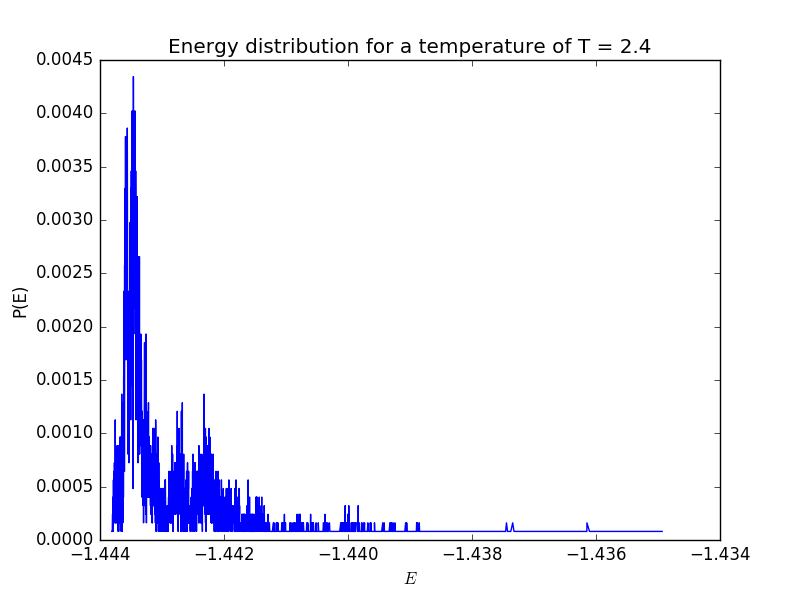
\includegraphics[scale=0.6]{PDF_T_24.png}
\caption{Configuration of the probability density function for energy for a lattice of $L = 20$. }\label{fig:pdf_24}
\end{figure}

\begin{figure}[H]
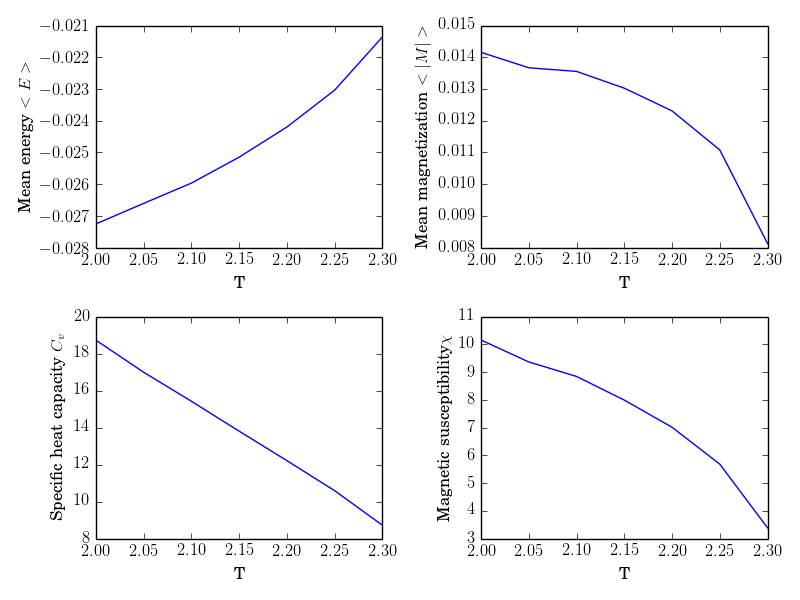
\includegraphics[scale=0.5]{exp_val40.png}
\caption{A set of two plots of expectation values for the energy and magnetization, aswell as two plots for the variances $C_v$ and $\chi$. All plots are represented as a function of a temperature development. The plots are for a lattice $L = 40$.}\label{fig:exp_40}
\end{figure}


\begin{figure}[H]
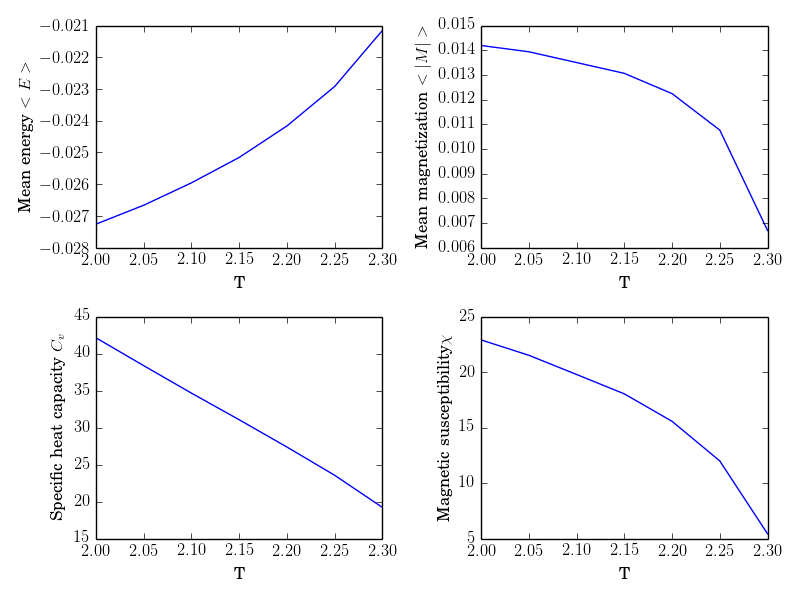
\includegraphics[scale=0.5]{exp_val60.png}
\caption{A set of two plots of expectation values for the energy and magnetization, aswell as two plots for the variances $C_v$ and $\chi$. All plots are represented as a function of a temperature development. The plots are for a lattice $L = 60$.}\label{fig:exp_60}
\end{figure}


\begin{figure}[H]
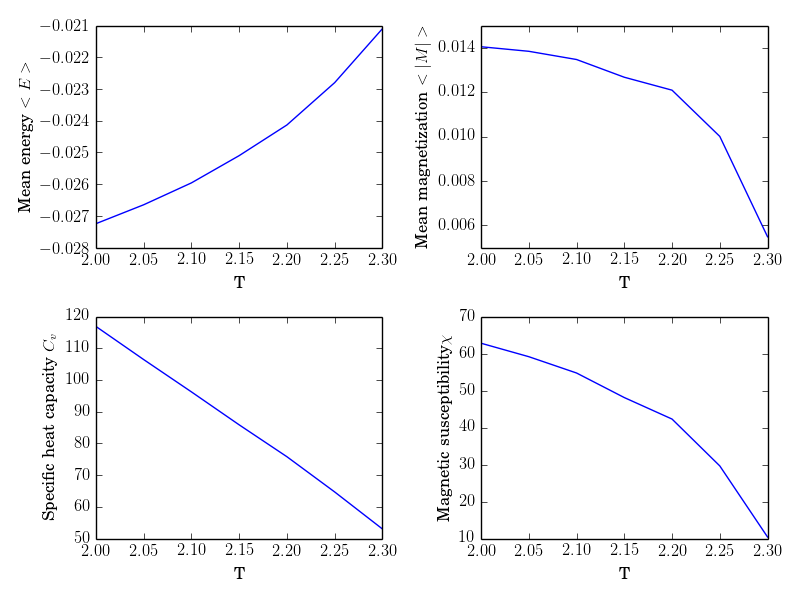
\includegraphics[scale=0.5]{exp_val100.png}
\caption{A set of two plots of expectation values for the energy and magnetization, aswell as two plots for the variances $C_v$ and $\chi$. All plots are represented as a function of a temperature development. The plots are for a lattice $L = 100$.}\label{fig:exp_100}
\end{figure}


\begin{figure}[H]
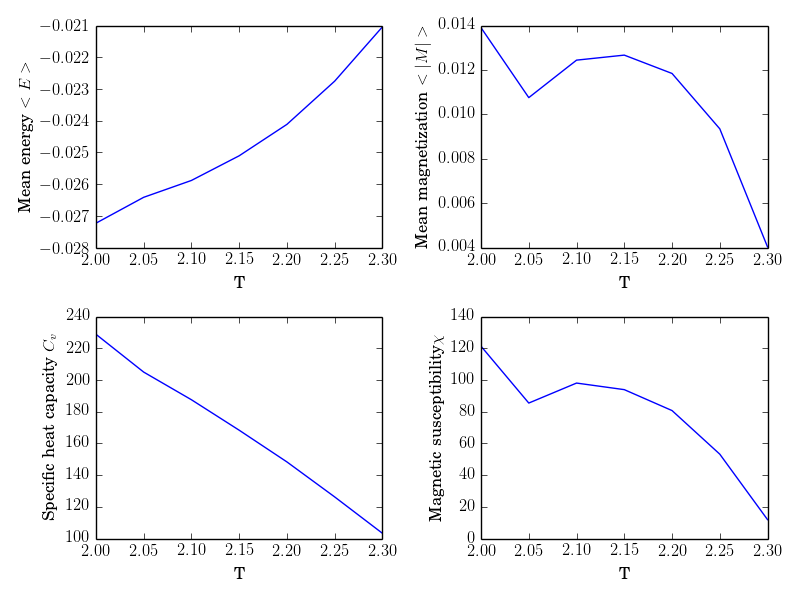
\includegraphics[scale=0.5]{exp_val140.png}
\caption{A set of two plots of expectation values for the energy and magnetization, aswell as two plots for the variances $C_v$ and $\chi$. All plots are represented as a function of a temperature development. The plots are for a lattice $L = 140$.}\label{fig:exp_140}
\end{figure}


\section{Discussion}

Considereing the results presented in the figures \ref{fig:exp_t1} through \ref{fig:exp_t2_ord} there is a strong indication the  equilibrium time occurs in the area around $10^5$ cycles, possibly lower for the very un-volatile configuration in figure \ref{fig:exp_t1}. Considering the behaviour of accepted configurations per cycle as a function of temperature in the system a systematic difference is found between the given temperatures. As shown by the figure \ref{fig:temp_config} the number of accepted configurations per cycle is increased significantly with temperature. This may be caused by an energy surplus in the  system causing more volatility as the system. \\
 
\noindent Looking at figure \ref{fig:accept_config} it seems there doesn't seem to be any correlation between initial state and number of accepted state per experiment. \\

\noindent The probability density plots in the figures \ref{fig:pdf_1} and \ref{fig:pdf_24} show that while the probability for finding the system in a state with the predicte steady state energy is nigh on zero, the probability of finding it in a close configuration is exceedingly large. There seems to be a good mapping between the probability distribution and the calculated expecation values for both $T=1$ and $T = 2.4$. Because of the above argument no consideration was made whether the  state started in an ordered or disordered configuration.\\

\noindent When observing the usefullness of parallellizing code an experiment was started for the case $L = 140$ which took about fourteen minutes to complete with parallellized code, but produced no output with a factor two increase for time in the unparallellized case. So time-wise it's a great investment to parallellize code with a number of FLOPs that go on magnitudes of $\approx 10^{10}$. Figures \ref{fig:exp_40} through \ref{fig:exp_140} show results from the computations with bigger lattices. Unfortunately the results seem rather unphysical in comparison to Lars Onsagers findings that would place the critical teperature $T_c$ at a temperature $T \approx 2.269$. As it stands there might be a problem in the computing that confound the data. There might be some interference aswell from the fact that the initially noisy data is not discounted in the computation of expecation values.
\section{Conclusion}

In this project analytical solutions for the $L =2$ case were compared with numerical results and found to be satisfyingly coherent. The numerical solution of the system was computed with a mersienne algorithm with a metropolist test as the principal logic. All systems tested with varying dimensionality showed convergence after a set of monte-carlo iterations. Furthermore computations were made on larger lattices of sizes up to $L = 140$ to determine the critical temperature of a phase change. Through these plots no clear evidence can be drawn on such a temperature. I sum it seems the implementation is at least partially successful and can be used to study steady states for thermodynamic systems of varying sizes
\end{document}